\documentclass[openany]{book}

\usepackage{etoolbox}
\usepackage{graphicx}
\graphicspath{ {./images/} }
\usepackage{subfig}

\makeatletter
\patchcmd{\@maketitle}{\newpage}{}{}{} 

\renewcommand{\@makeschapterhead}[1]{
	{\noindent\raggedright\normalfont
		\huge\bfseries 
		#1\par\nobreak}
	\vspace{\baselineskip}
}

\makeatother

\begin{document}

\author{https://github.com/HilalNazli/AcilDurumCantasiHK}
\title{Acil Durum Çantası\\Hazırlama Klavuzu}
\date{Mart 2023\\v1.0.0}

\maketitle

\chapter*{Giriş}

Acil durum çantası; deprem, sel gibi afetler veya herhangi bir başka sebeple evimizde barınamayacağımız durumlarda, bize yardım ulaşana kadarki süreçte hayatımızı sağlıklı bir şekilde sürdürebilmemiz için gerekli malzemeleri içeren çantadır. Bu klavuz, acil durum çantasında bulunması gereken malzemeler ve kullanım şekilleri hakkında bilgilendirme amacı ile hazırlanmıştır.

\vspace{2ex}
\title{\textbf{Sorumluluk Reddi}}

Bu klavuzun içeriği yalnızca genel bilgi verme amaçlı olup, acil durumlarda tüm ihtiyaçları karşılama konusunda herhangi bir garanti vermemektedir. Bu klavuz doğrultusunda hazırlanacak acil durum çantasının kullanımına dair her türlü risk kullanıcıya aittir.
\chapter*{Çanta İçerik Grupları}

\centering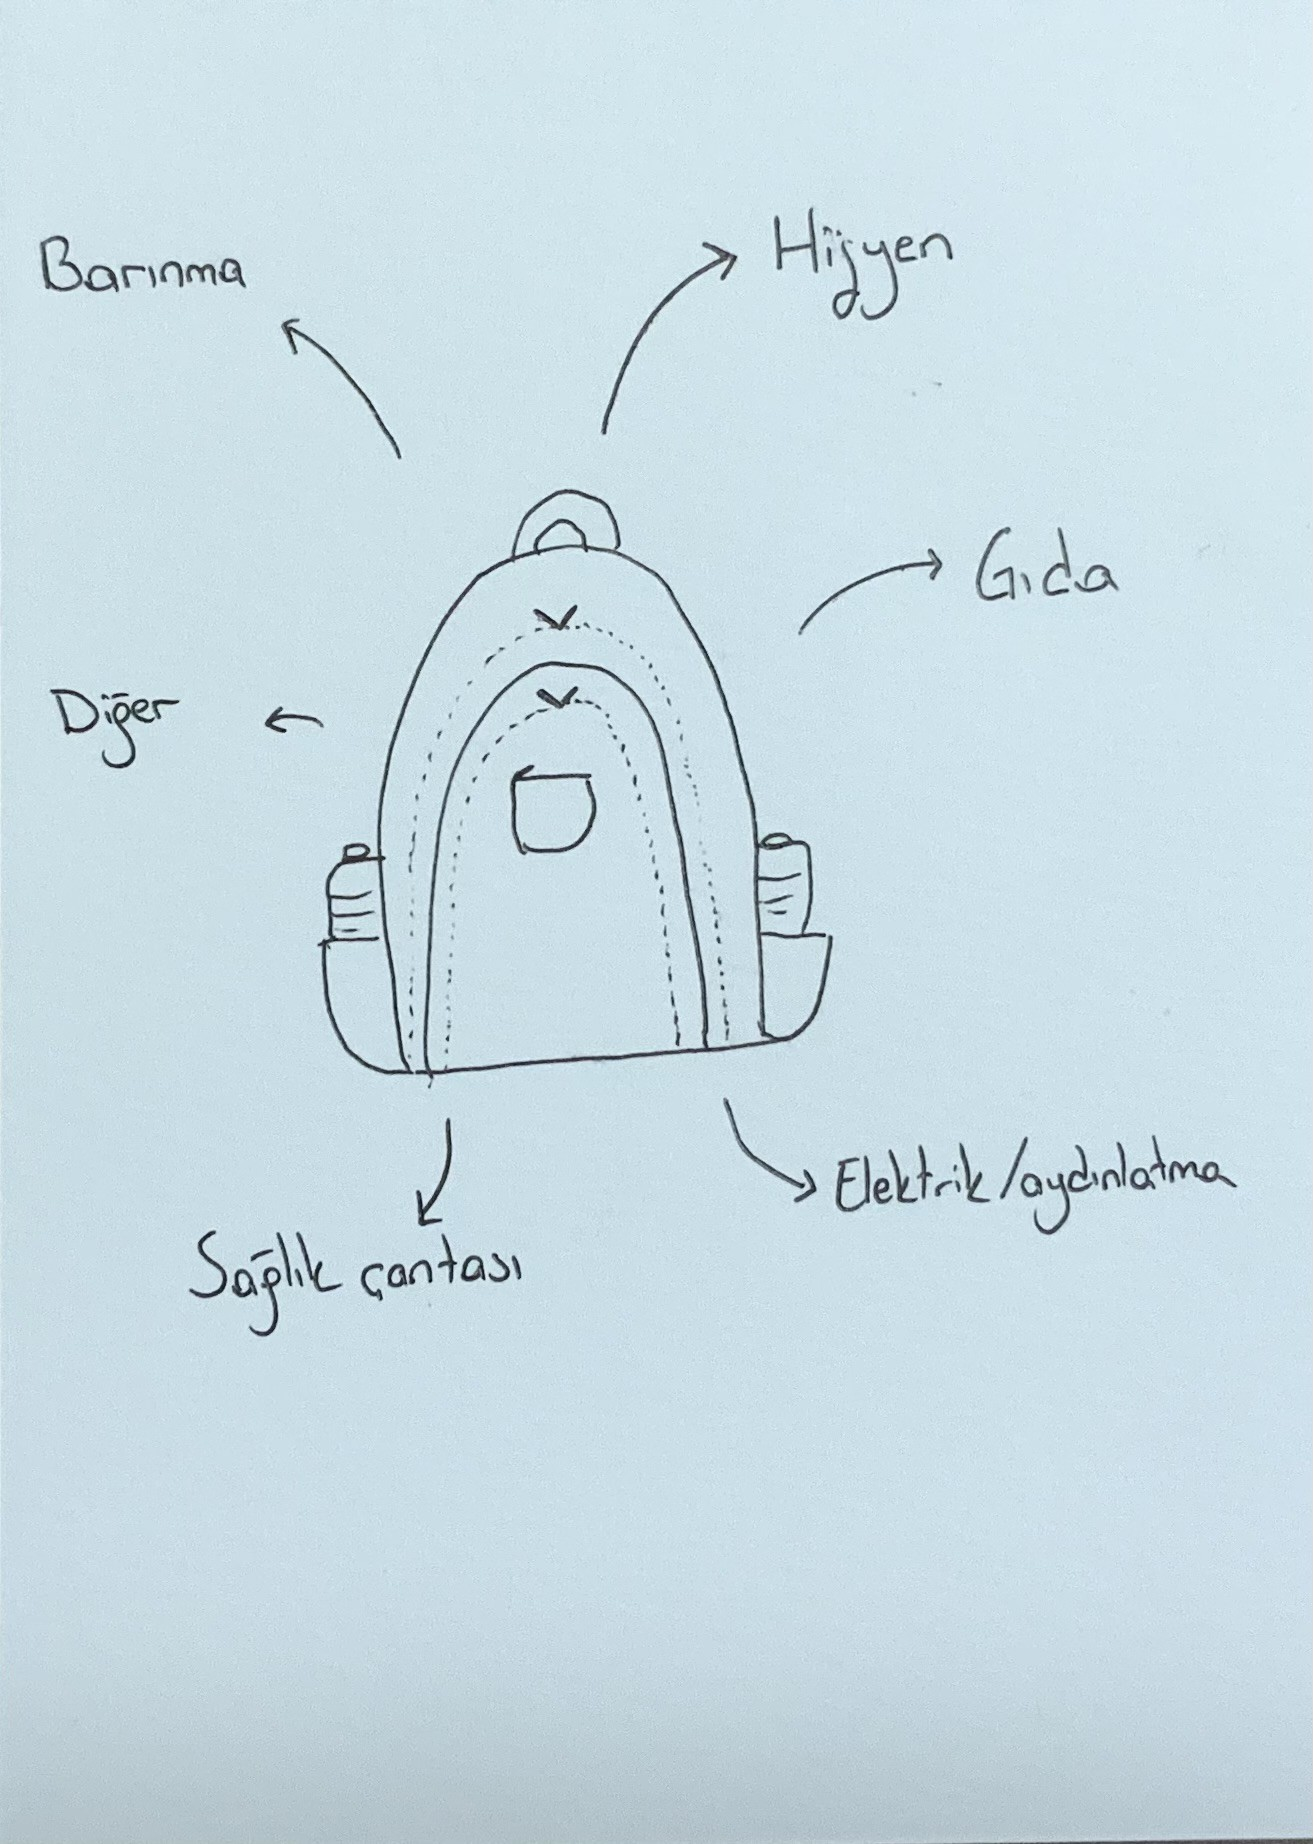
\includegraphics[width=\textwidth, 
                 height = 0.75\textheight, 
                 keepaspectratio]
                {bagContents.jpg}

\chapter*{Hijyen}

\begin{itemize}
	\item Acil durum tuvaleti (kişi sayısı x 5 adet x 1-3 gün)
	\item Tuvalet kağıdı
	\item Diş fırçası, diş macunu, diş ipi
	\item Sabun
	\item Alkollü/alkolsüz ıslak mendil
	\item Maske
	\item Poşet
	\item Tırnak makası
	\item Krem deodorant
	\item Kadın hijyen ürünleri
\end{itemize}

\centering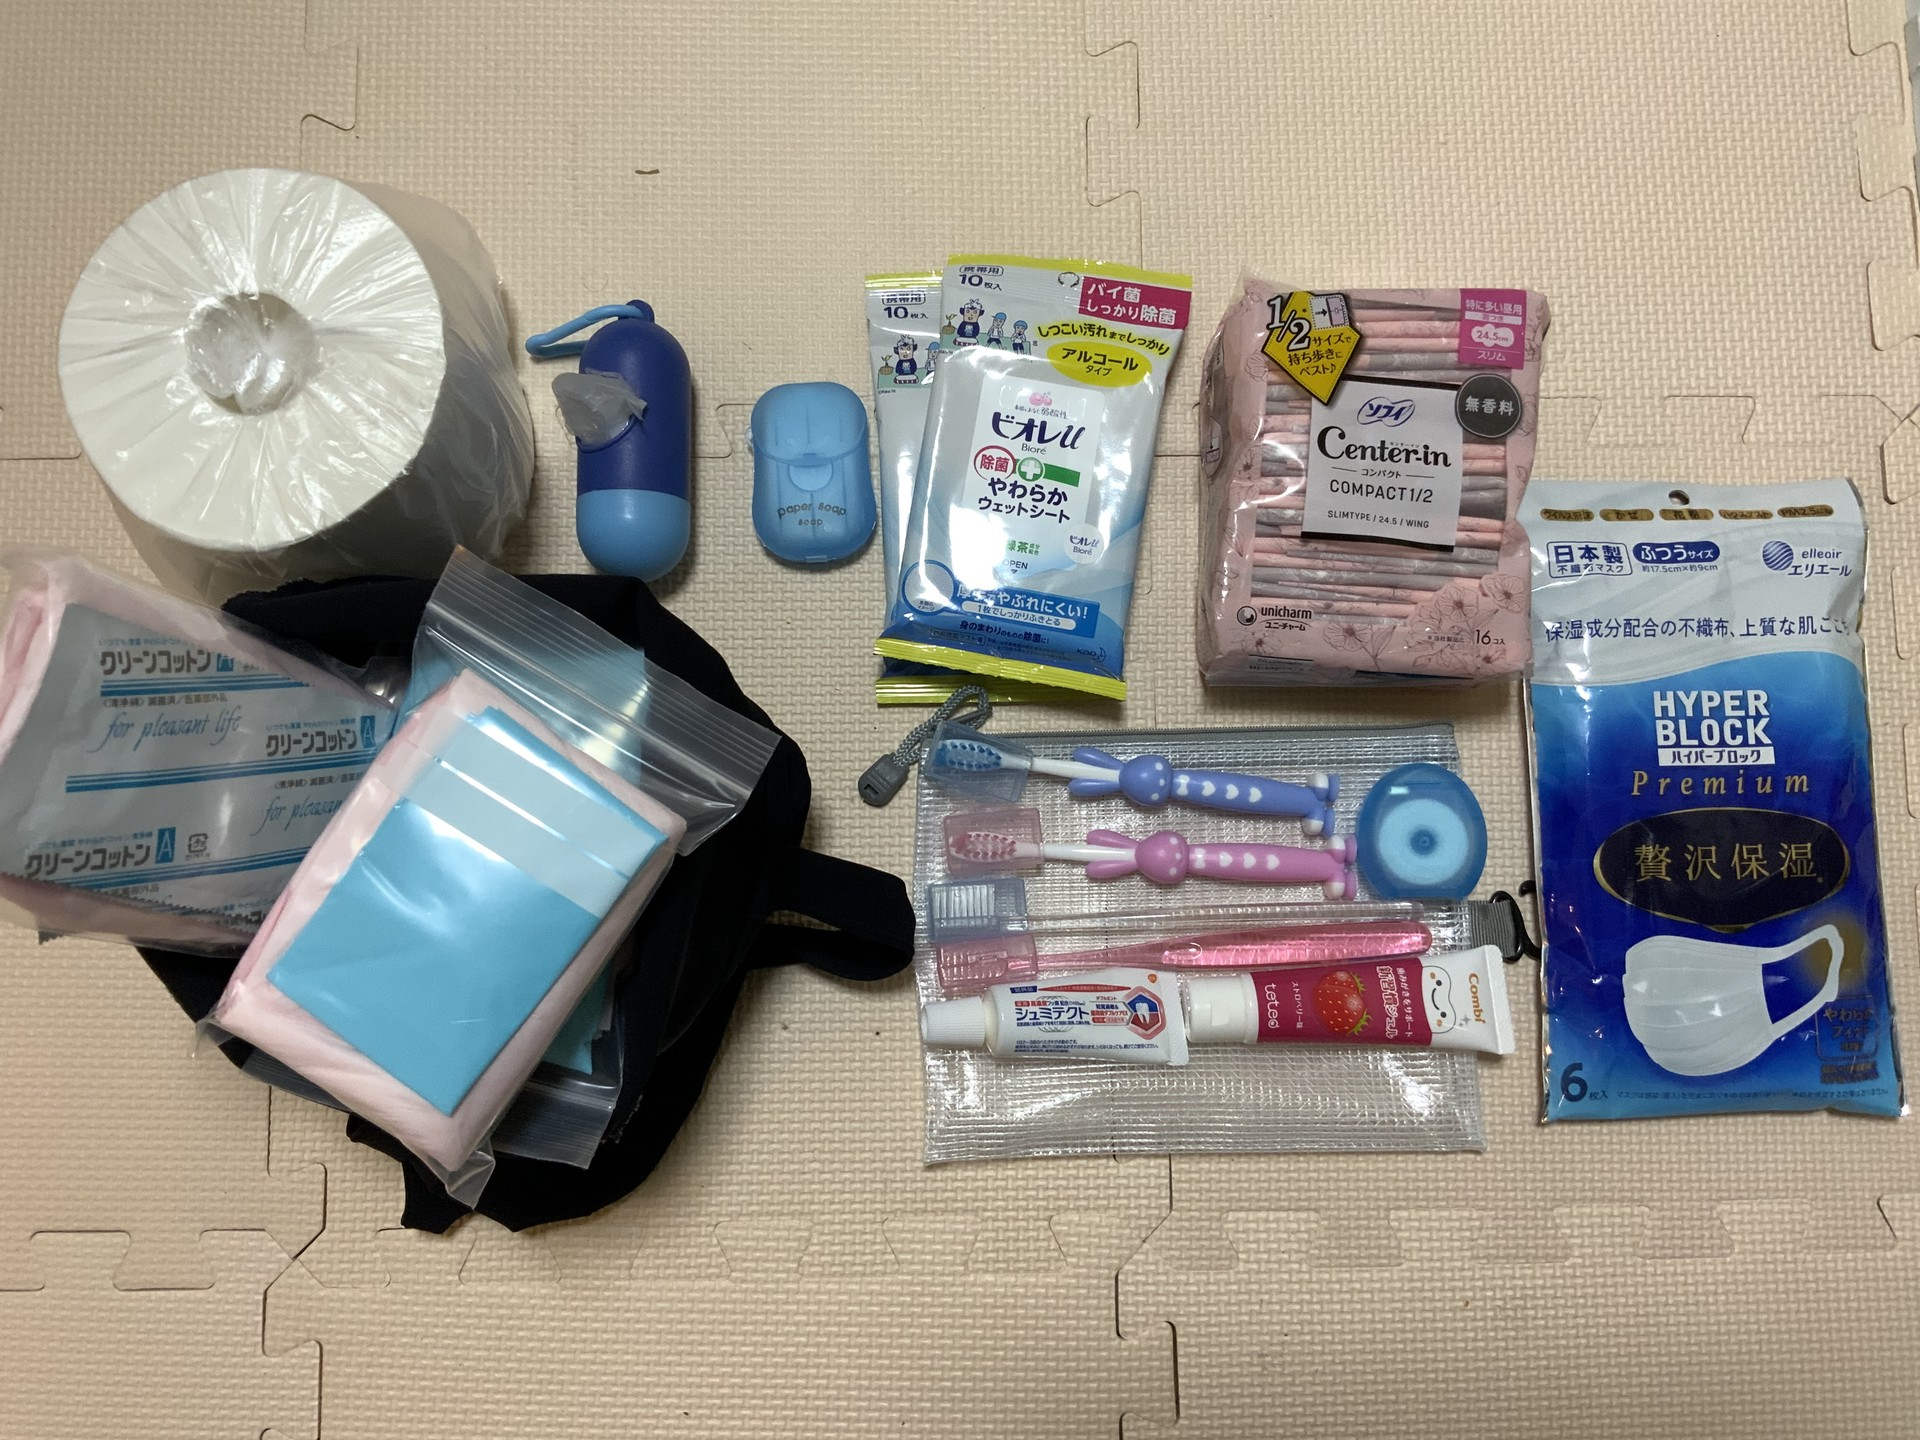
\includegraphics[width=\textwidth, 
height = 0.75\textheight, 
keepaspectratio]
{hygiene.jpg}

\chapter*{Acil Durum Tuvaleti}
\chapter*{Gıda}
\chapter*{Barınma}

\begin{itemize}
	\item İç çamaşırı (1-3 günlük)
	\item Bir set yedek kıyafet (kişi sayısınca, mevsime uygun)
	\item Acil durum battaniyesi (kişi sayısınca)
	\item Yağmurluk (kişi sayısınca)
	\item El yüz havlusu (kişi sayısınca)
\end{itemize}

\chapter*{Elektrik/Aydınlatma}

\begin{itemize}
	\item Fener
	\item Pil
	\item Taşınabilir şarj (powerbank)
	\item Şarj adaptörü
	\item USB kablo
	\item Radyo
	\item Şarjlı pil ve şarj cihazı
	\item Mum
\end{itemize}


\centering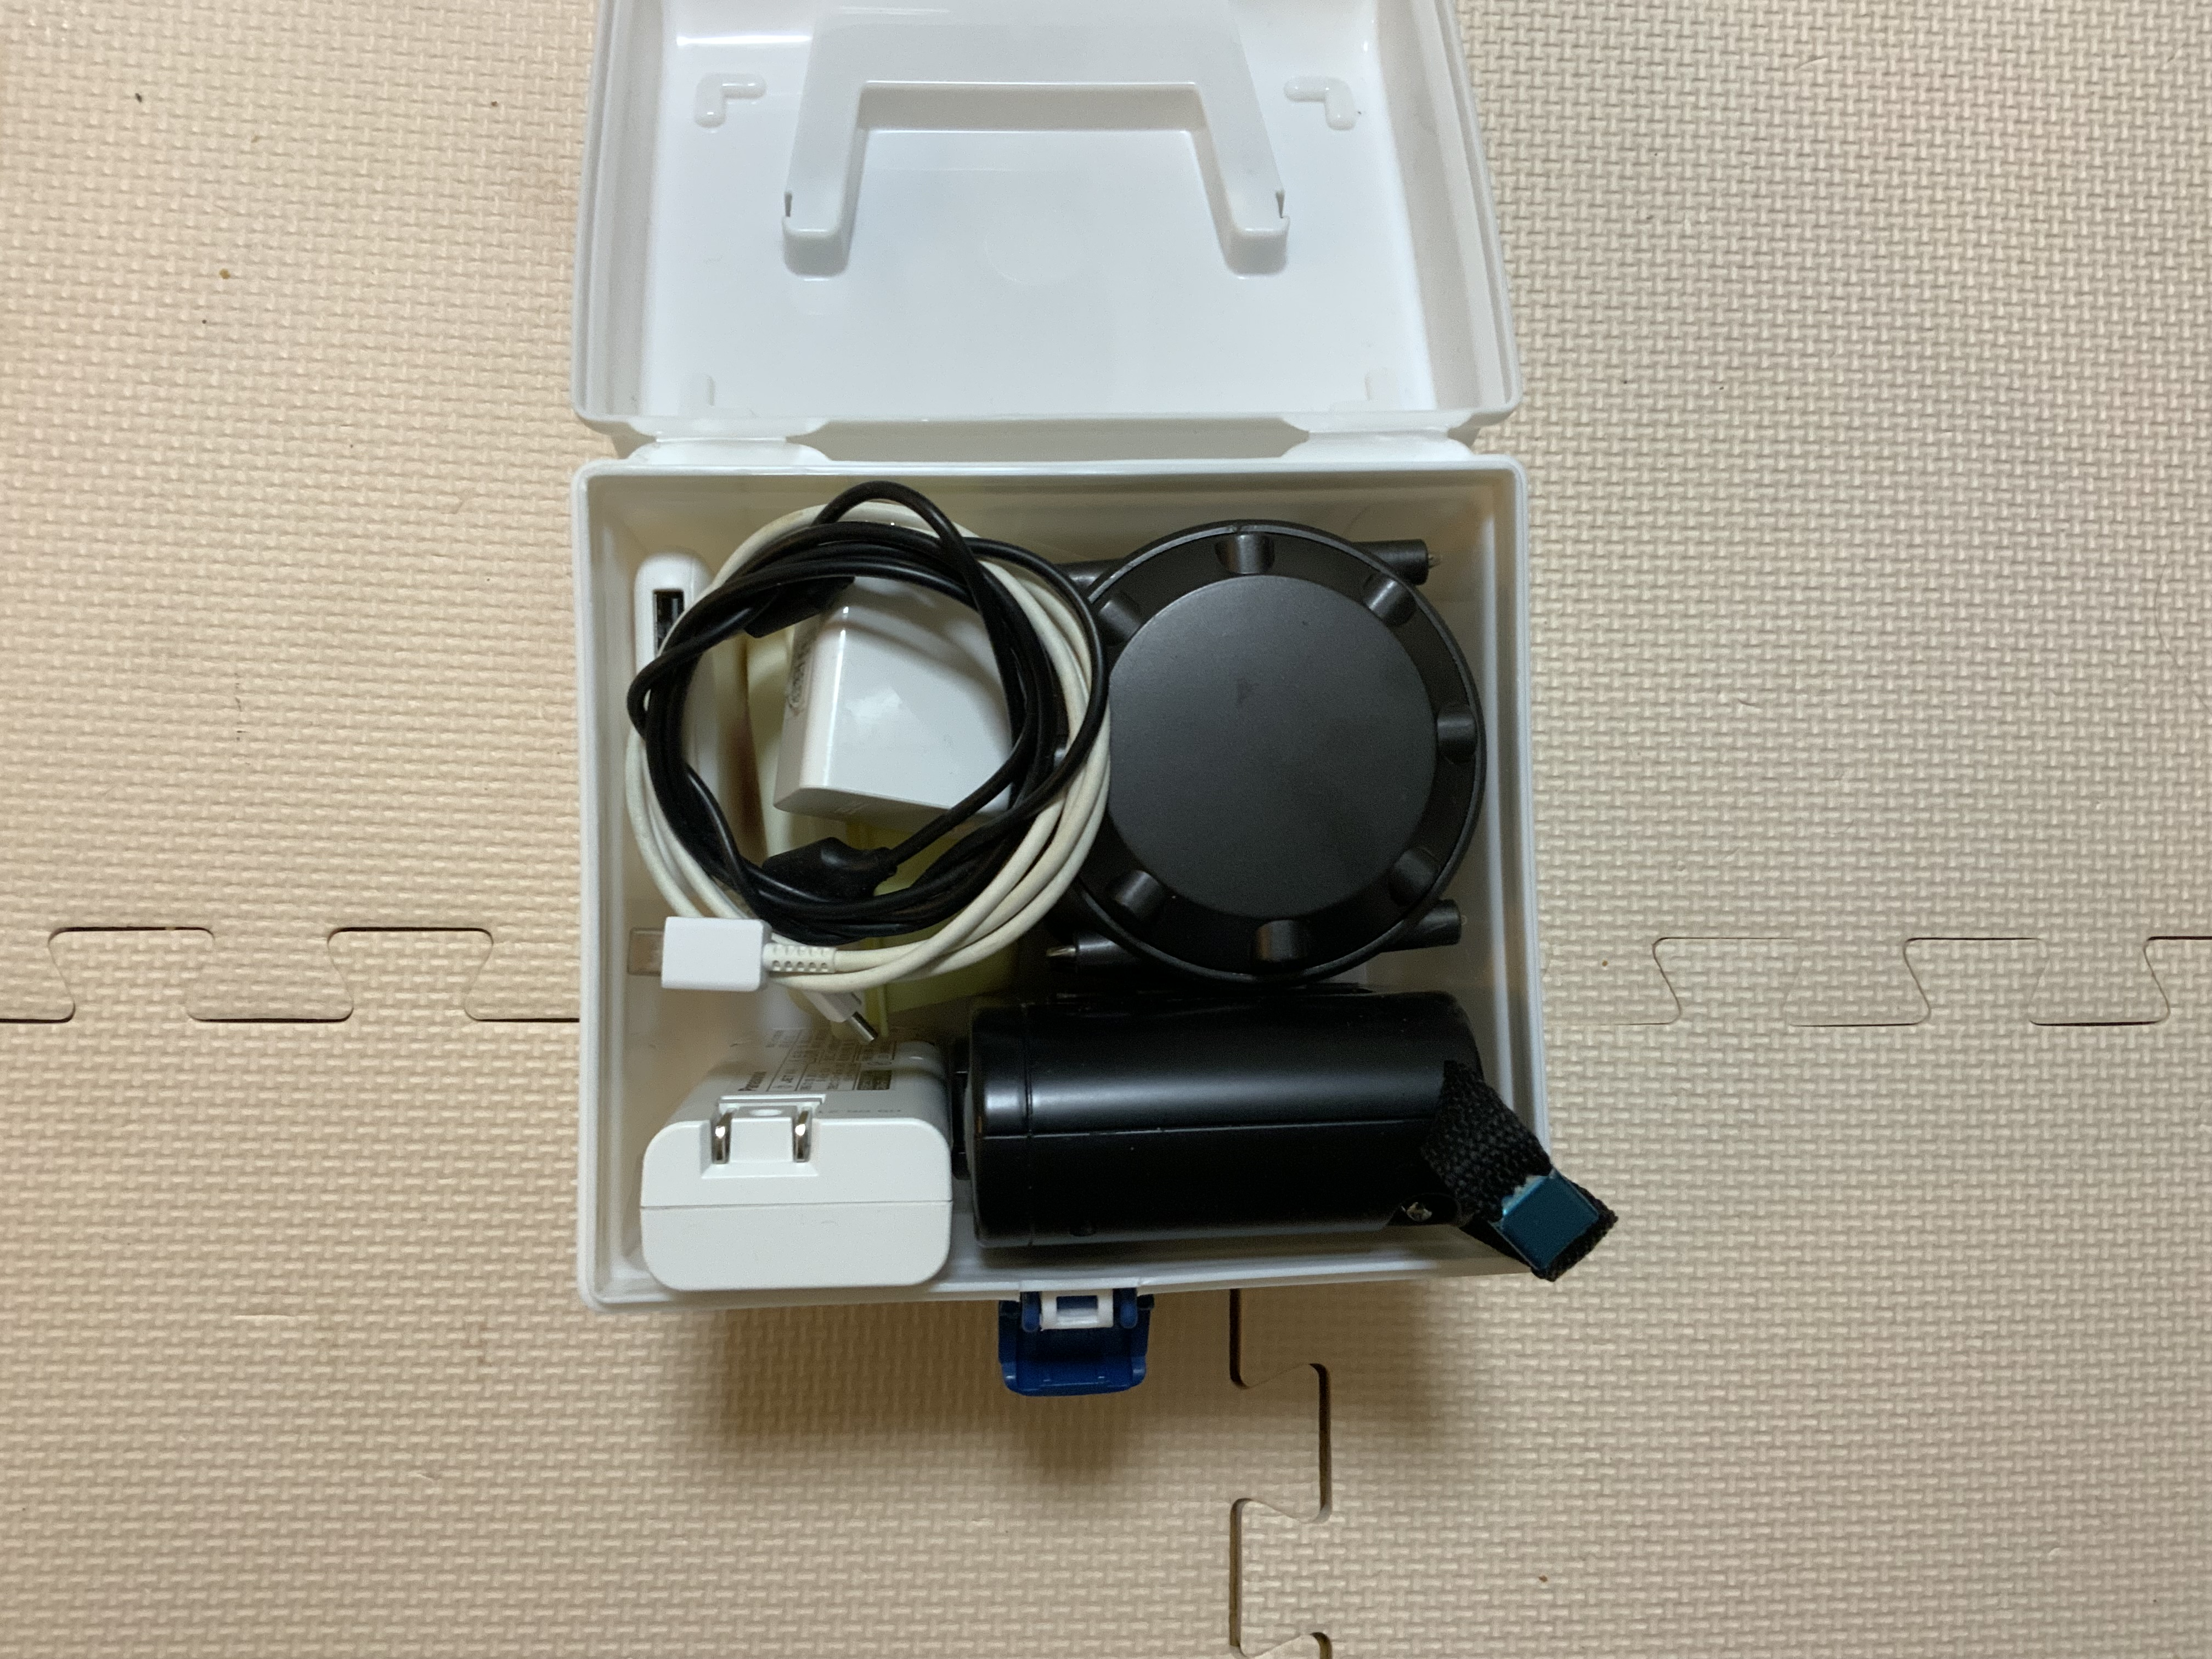
\includegraphics[width=\textwidth, 
height = 0.32\textheight, 
keepaspectratio]
{electrics01}

\centering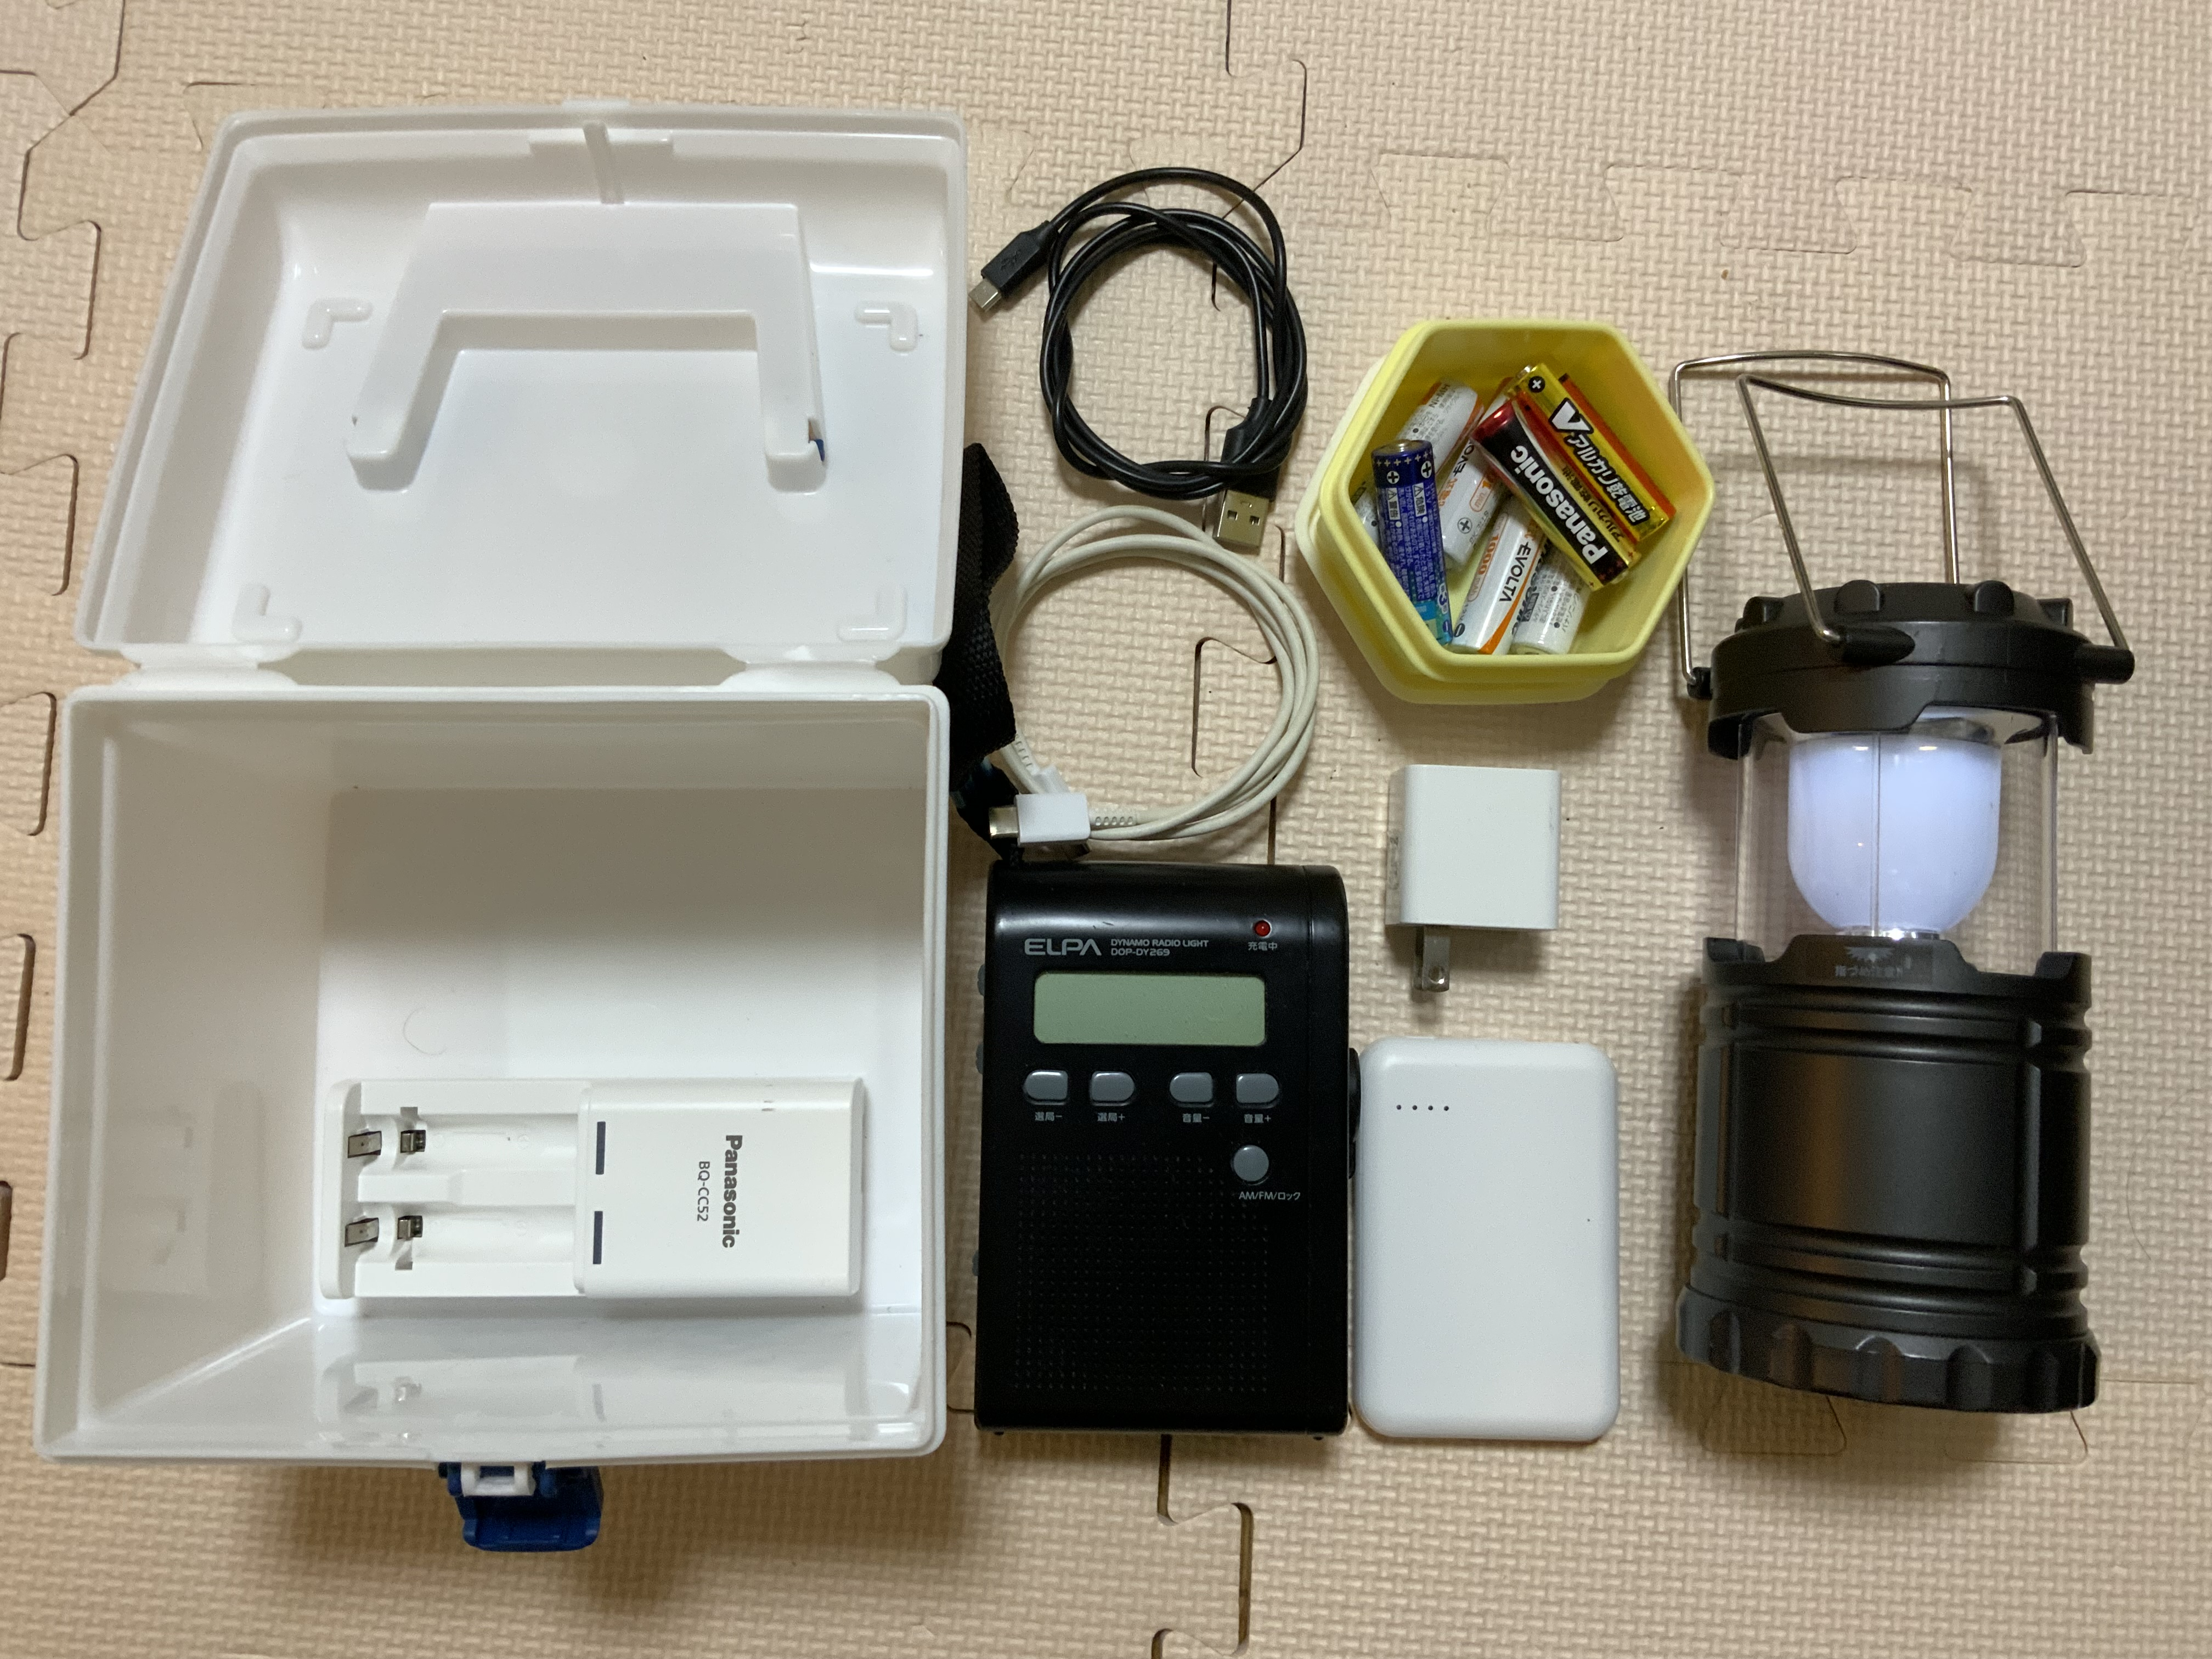
\includegraphics[width=\textwidth, 
height = 0.32\textheight, 
keepaspectratio]
{electrics02}

\chapter*{Sağlık Çantası}

\begin{itemize}
	\item Gazlı bez (bir kaç çeşit)
	\item Sargı bezi
	\item Üçgen sargı bezi
	\item Alkollü ıslak mendil (Yaraya müdahaleden önce ellerin temizlenmesi için. Yaraya temas ettirilmeyecek.)
	\item Sabun
	\item Oxydol (yaranın dezenfeksiyonu için)
	\item Pamuk
	\item Antibakteriyel krem (Furasin vb.)
	\item Ağrı kesici (yetişkin için ve çocuk için)
	\item Ateş düşürücü (yetişkin için ve çocuk için)
	\item Işık
	\item Yanık kremi (Yanık akan suda uzun süre tutulduktan sonra sürülecek. Yanık kreminin ağrı kesici özelliği yok ise ayrıca ağrı kesici krem (Anestol vb.))
	\item Antihistaminik krem (allerji veya böcek ısırması durumları için)
	\item Allerji ilacı (antihistamin)
	\item Mendil
	\item Çöp poşeti
	\item Eldiven
	\item Yara bandı
	\item Makas
	\item Cımbız
	\item Buz kesesi veya instant ice pack
	\item Alna yapıştırılan soğutucu (ateşlenme için)
	\item Acil durum numarasının yazılı olduğu kağıt
\end{itemize}

\centering\includegraphics[width=\textwidth, 
height = 0.7\textheight, 
keepaspectratio]
{firstAid}

\chapter*{Diğer}

\begin{itemize}
	\item Kimlik/pasaport fotokopileri
	\item Nakit para
	\item Evden en yakın toplanma alanına giden yol haritası
	\item Yakınların telefon numaraları ve açık adresleri
	\item Çakmak (çocuk varsa kilitli)
	\item Çakı
	\item Kalem, defter
	\item Düdük (yardım çağırmak için)
	\item Yedek gözlük
	\item Küçük sağlam kürek (toprağı kazmak için)
	\item İş eldiveni
	\item Su taşıma poşeti
	\item İp (çamaşır asma, eşyaları gruplayıp taşıma, barınak kurma vb. için)
\end{itemize}
\chapter*{Bebekli/Küçük Çocuklu Aileler İçin}

\begin{itemize}
	\item Formül süt
	\item Biberon
	\item Hazır ek gıda
	\item Küçük kaşık
	\item Bez
	\item Pişik kremi
	\item Islak mendil
	\item Poşet
	\item Suluk
	\item Battaniye
\end{itemize}

\backmatter
% bibliography, glossary and index would go here.

\end{document}